% =====================================================================
%  Лекция 8. Доверительные интервалы. Асимптотические доверительные интервалы
%  Дата: 2026-11-05
% =====================================================================
\section{Доверительные интервалы}
\label{lec:08}

\subsection{Определения}
\label{lec08:definitions}

Точечная оценка даёт одно число, но ничего не говорит о том, насколько ей можно доверять.
Доверительный интервал~--- это интервал со случайными концами, который накрывает
неизвестный параметр с заданной вероятностью.

Пусть $\xi$~--- генеральная совокупность с функцией распределения $F_\xi(x, \theta)$,
$\theta \in \Th \subset \R$, и $X_{[n]} = (X_1, \ldots, X_n)$~--- выборка.

\begin{definition}
  Пусть $\epsilon \in (0, 1)$ и существуют статистики $S^-(X_{[n]}, \epsilon)$ и
  $S^+(X_{[n]}, \epsilon)$ такие, что
  \[
    \P\bigl\{S^-(X_{[n]}, \epsilon) < \theta < S^+(X_{[n]}, \epsilon)\bigr\} = 1 - \epsilon.
  \]
  Тогда интервал $\bigl(S^-(X_{[n]}, \epsilon), S^+(X_{[n]}, \epsilon)\bigr)$ называется
  \emph{доверительным интервалом} для параметра~$\theta$ с \emph{уровнем доверия} $1 - \epsilon$.
\end{definition}

\begin{definition}
  Если вместо равенства выполнено
  \[
    \P\bigl\{S^-(X_{[n]}, \epsilon) < \theta < S^+(X_{[n]}, \epsilon)\bigr\}
    \xrightarrow[n \to \infty]{} 1 - \epsilon,
  \]
  то интервал называется \emph{асимптотическим} (приближённым) доверительным интервалом
  с уровнем доверия $1 - \epsilon$.
\end{definition}

\begin{remark}
  Случайны здесь концы интервала, а не $\theta$: параметр~--- неизвестное, но фиксированное
  число. <<Уровень доверия $0{,}95$>> означает, что интервал, построенный по случайной выборке,
  накрывает истинное~$\theta$ с вероятностью $0{,}95$.
\end{remark}

\subsection{Асимптотический доверительный интервал по асимптотически нормальной оценке}
\label{lec08:asymptotic}

Пусть $\hat\theta$~--- асимптотически нормальная оценка параметра~$\theta$ с коэффициентом
$\sigma^2(\theta)$ (раздел~\ref{lec06:asymptotic-normality}):
\[
  \sqrt{n}\,(\hat\theta - \theta) \tod \zeta \sim \Norm\bigl(0, \sigma^2(\theta)\bigr).
\]
Будем считать, что функция $\sigma^2(\theta)$ непрерывна на~$\Th$ и не обращается в ноль.

Поделив на $\sigma(\theta)$, получили бы величину, сходящуюся к $\Norm(0, 1)$. Но $\sigma(\theta)$
зависит от неизвестного~$\theta$, и интервал из этого не построишь. Идея~--- заменить
$\sigma(\theta)$ на $\sigma(\hat\theta)$. Чтобы это обосновать, нужны два факта.

\begin{reminder}[Сходимость по распределению]
  \begin{itemize}
    \item $\eta_n \tod \eta \iff F_{\eta_n}(x) \to F_\eta(x)$ в каждой точке непрерывности~$F_\eta$.
    \item Распределение, функция распределения и характеристическая функция
          $\phi_\eta(t) = \E e^{it\eta}$ однозначно определяют друг друга:
          $\P_\eta \leftrightarrow F_\eta \leftrightarrow \phi_\eta$. Сходимость по распределению
          равносильна поточечной сходимости характеристических функций.
  \end{itemize}
\end{reminder}

\begin{theorem}[о непрерывности]
  \label{lec08:continuity}
  Пусть $\eta_n$, $\eta$~--- случайные векторы, $\eta_n \tod \eta$, и $H$~--- непрерывная функция.
  Тогда $H(\eta_n) \tod H(\eta)$.
\end{theorem}

\begin{lemma}[{\cite[гл.~16, лемма~1.1]{bure}}]
  \label{lec08:joint}
  Если $\sqrt{n}\,(\hat\theta - \theta) \tod \zeta \sim \Norm(0, \sigma^2(\theta))$, то случайный вектор
  \[
    \bigl(\sqrt{n}\,(\hat\theta - \theta),\ \hat\theta\bigr) \tod (\zeta, \theta).
  \]
\end{lemma}

\begin{addendum}
  \emph{Идея доказательства леммы} \cite[гл.~16, лемма~1.1]{bure}. Достаточно проверить
  сходимость характеристических функций. Так как
  $\hat\theta = \theta + \frac{1}{\sqrt n} \cdot \sqrt{n}\,(\hat\theta - \theta)$,
  \[
    \E e^{i t_1 \sqrt{n}(\hat\theta - \theta) + i t_2 \hat\theta}
    = e^{i t_2 \theta}\, \phi_{\sqrt{n}(\hat\theta - \theta)}\Bigl(t_1 + \frac{t_2}{\sqrt n}\Bigr)
    \xrightarrow[n \to \infty]{} e^{i t_2 \theta}\, \phi_\zeta(t_1) = \E e^{i t_1 \zeta + i t_2 \theta}.
  \]
  Переход к пределу законен, потому что характеристические функции сходятся равномерно на
  отрезках, а $\phi_\zeta$ непрерывна.
\end{addendum}

Теперь применим теорему~\ref{lec08:continuity} к функции
\[
  H(x_1, x_2) = \frac{x_1}{\sigma(x_2)},
\]
она непрерывна, так как $\sigma$ непрерывна и не равна нулю. По лемме~\ref{lec08:joint}
\[
  H\bigl(\sqrt{n}\,(\hat\theta - \theta), \hat\theta\bigr)
  = \frac{\sqrt{n}\,(\hat\theta - \theta)}{\sigma(\hat\theta)}
  \tod H(\zeta, \theta) = \frac{\zeta}{\sigma(\theta)}.
\]
Если $\zeta \sim \Norm(0, \sigma^2)$, то $\frac1\sigma \zeta \sim \Norm\bigl(0, \frac{\sigma^2}{\sigma^2}\bigr) = \Norm(0, 1)$.
Итак,
\begin{equation}
  \label{lec08:eq:pivot}
  \frac{\sqrt{n}\,(\hat\theta - \theta)}{\sigma(\hat\theta)} \tod \zeta' \sim \Norm(0, 1).
\end{equation}

\subsubsection{Построение интервала}

Пусть $z_p$~--- квантиль уровня~$p$ стандартного нормального распределения: $\Phi(z_p) = p$,
где $\Phi$~--- функция распределения $\Norm(0, 1)$. Разобьём $\epsilon = \epsilon_1 + \epsilon_2$
и отрежем от нормальной кривой хвосты площадью $\epsilon_1$ слева и $\epsilon_2$ справа
(\cref{lec08:fig:tails}). Из~\eqref{lec08:eq:pivot}
\[
  \P\biggl\{ z_{\epsilon_1} < \frac{\sqrt{n}\,(\hat\theta - \theta)}{\sigma(\hat\theta)} < z_{1 - \epsilon_2} \biggr\}
  \xrightarrow[n \to \infty]{} \Phi(z_{1-\epsilon_2}) - \Phi(z_{\epsilon_1}) = (1 - \epsilon_2) - \epsilon_1 = 1 - \epsilon.
\]
Обычно берут симметричный вариант $\epsilon_1 = \epsilon_2 = \frac\epsilon2$. Нормальная плотность
симметрична, поэтому $z_{\epsilon/2} = -z_{1 - \epsilon/2}$, и
\[
  -z_{1 - \frac\epsilon2} < \frac{\sqrt{n}\,(\hat\theta - \theta)}{\sigma(\hat\theta)} < z_{1 - \frac\epsilon2}.
\]
Выражая отсюда~$\theta$, получаем
\[
  \hat\theta - z_{1 - \frac\epsilon2} \frac{\sigma(\hat\theta)}{\sqrt n}
  < \theta <
  \hat\theta + z_{1 - \frac\epsilon2} \frac{\sigma(\hat\theta)}{\sqrt n}.
\]

\begin{keybox}[Асимптотический доверительный интервал]
  Если $\hat\theta$ асимптотически нормальна с коэффициентом $\sigma^2(\theta)$ (непрерывным
  и ненулевым), то
  \[
    \biggl( \hat\theta - z_{1 - \frac\epsilon2} \frac{\sigma(\hat\theta)}{\sqrt n},\ \
            \hat\theta + z_{1 - \frac\epsilon2} \frac{\sigma(\hat\theta)}{\sqrt n} \biggr)
  \]
  ~--- асимптотический доверительный интервал для~$\theta$ с уровнем доверия $1 - \epsilon$.
\end{keybox}

Например, при $\epsilon = 0{,}05$ квантиль $z_{0{,}975} \approx 1{,}96$.

\begin{figure}[h]
  \centering
  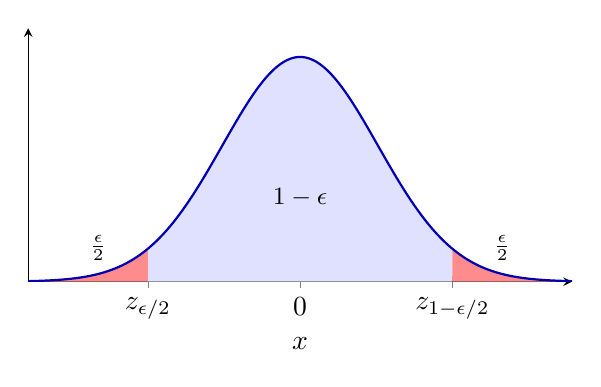
\begin{tikzpicture}
    \begin{axis}[
      width=0.7\textwidth, height=4.8cm,
      xmin=-3.5, xmax=3.5, ymin=0, ymax=0.45,
      axis lines=left, xlabel={$x$}, ylabel={},
      xtick={-1.96, 0, 1.96},
      xticklabels={$z_{\epsilon/2}$, $0$, $z_{1-\epsilon/2}$},
      ytick=\empty,
    ]
      \addplot[fill=blue!12, draw=none, domain=-1.96:1.96, samples=80]
        {exp(-x^2/2)/sqrt(2*pi)} \closedcycle;
      \addplot[fill=red!45, draw=none, domain=-3.5:-1.96, samples=40]
        {exp(-x^2/2)/sqrt(2*pi)} \closedcycle;
      \addplot[fill=red!45, draw=none, domain=1.96:3.5, samples=40]
        {exp(-x^2/2)/sqrt(2*pi)} \closedcycle;
      \addplot[thick, blue!70!black, domain=-3.5:3.5, samples=150] {exp(-x^2/2)/sqrt(2*pi)};
      \node[font=\small] at (axis cs:0, 0.15) {$1 - \epsilon$};
      \node[font=\small] at (axis cs:-2.6, 0.06) {$\frac\epsilon2$};
      \node[font=\small] at (axis cs:2.6, 0.06) {$\frac\epsilon2$};
    \end{axis}
  \end{tikzpicture}
  \caption{Плотность $\Norm(0, 1)$: между квантилями $z_{\epsilon/2} = -z_{1-\epsilon/2}$ и
           $z_{1-\epsilon/2}$ лежит площадь $1 - \epsilon$, в каждом хвосте~--- $\frac\epsilon2$.}
  \label{lec08:fig:tails}
\end{figure}

\subsection{Примеры}
\label{lec08:examples}

Во всех примерах асимптотическая нормальность получается из центральной предельной теоремы.

\begin{reminder}[Центральная предельная теорема]
  Пусть $\xi_1, \xi_2, \ldots$ независимы, одинаково распределены, $\E\xi_k = a$,
  $\D\xi_k = \sigma^2 < \infty$. Тогда
  \[
    \frac{1}{\sqrt n} \sum_{k=1}^n (\xi_k - a) \tod \zeta \sim \Norm(0, \sigma^2).
  \]
\end{reminder}

В частности, для выборочного среднего
$\sqrt{n}\,(\Xbar - \E\xi) = \frac{1}{\sqrt n} \sum_{i=1}^n (X_i - \E\xi) \tod \Norm(0, \D\xi)$:
$\Xbar$~--- асимптотически нормальная оценка $\E\xi$ с коэффициентом $\sigma^2 = \D\xi$.

\begin{example}[распределение Пуассона]
  \label{lec08:ex:pois}
  $\xi \sim \Pois(\alpha)$, $\theta = \alpha$. ОМП~--- выборочное среднее: $\hat\alpha = \Xbar$
  (пример~\ref{lec07:ex:mle-pois}). Так как $\E\xi = \D\xi = \alpha$, по ЦПТ
  \[
    \sqrt{n}\,(\hat\alpha - \alpha) = \frac{1}{\sqrt n} \sum_{i=1}^n (X_i - \alpha) \tod \zeta \sim \Norm(0, \alpha),
  \]
  то есть $\hat\alpha$ асимптотически нормальна с коэффициентом $\sigma^2(\alpha) = \alpha$.
  Отсюда $\sigma(\alpha) = \sqrt\alpha$, $\sigma(\hat\alpha) = \sqrt{\Xbar}$, и асимптотический
  доверительный интервал:
  \[
    \biggl( \Xbar - z_{1 - \frac\epsilon2} \sqrt{\frac{\Xbar}{n}},\ \
            \Xbar + z_{1 - \frac\epsilon2} \sqrt{\frac{\Xbar}{n}} \biggr).
  \]
\end{example}

\begin{example}[показательное распределение]
  \label{lec08:ex:exp}
  $\xi \sim \Exp(\lambda)$: $\E\xi = \frac1\lambda$, $\D\xi = \frac{1}{\lambda^2}$, ОМП
  $\hat\lambda = \frac{1}{\Xbar}$. Удобнее построить интервал не для самого~$\lambda$, а для
  функции от него, $\theta = \frac1\lambda = \E\xi$. Отображение $\lambda \mapsto \frac1\lambda$
  взаимно однозначно, поэтому по инвариантности ОМП (утверждение~\ref{lec07:invariance})
  оценка максимального правдоподобия для~$\theta$~--- это $\hat\theta = \frac{1}{\hat\lambda} = \Xbar$,
  и по ЦПТ
  \[
    \sqrt{n}\,\Bigl(\Xbar - \frac1\lambda\Bigr) = \frac{1}{\sqrt n} \sum_{i=1}^n \Bigl(X_i - \frac1\lambda\Bigr)
    \tod \zeta \sim \Norm\Bigl(0, \frac{1}{\lambda^2}\Bigr).
  \]
  Коэффициент как функция параметра $\theta = \frac1\lambda$: $\sigma^2(\theta) = \theta^2$,
  $\sigma(\theta) = \theta$, поэтому $\sigma(\hat\theta) = \Xbar$. Асимптотический доверительный
  интервал для $\frac1\lambda$:
  \[
    \biggl( \Xbar - z_{1 - \frac\epsilon2} \frac{\Xbar}{\sqrt n},\ \
            \Xbar + z_{1 - \frac\epsilon2} \frac{\Xbar}{\sqrt n} \biggr).
  \]
\end{example}

\begin{addendum}
  Проверим, что $\hat\lambda = \frac1\Xbar$ действительно ОМП (на лекции это не выводилось):
  $f_\xi(x, \lambda) = \lambda e^{-\lambda x}$ при $x \ge 0$, поэтому
  $\ln L = n \ln\lambda - \lambda \sum_{i=1}^n X_i$ и
  $\frac{\partial \ln L}{\partial \lambda} = \frac{n}{\lambda} - \sum_{i=1}^n X_i = 0$ даёт
  $\hat\lambda = \frac{1}{\Xbar}$; вторая производная $-\frac{n}{\lambda^2} < 0$.

  \smallskip
  Из интервала для $\frac1\lambda$ легко получить интервал для самого~$\lambda$: функция
  $t \mapsto \frac1t$ монотонна, поэтому (при $z_{1-\epsilon/2} < \sqrt n$)
  \[
    \frac1\lambda \in \Bigl( \Xbar\bigl(1 - \tfrac{z}{\sqrt n}\bigr),\ \Xbar\bigl(1 + \tfrac{z}{\sqrt n}\bigr) \Bigr)
    \iff
    \lambda \in \biggl( \frac{1}{\Xbar\,(1 + z/\sqrt n)},\ \frac{1}{\Xbar\,(1 - z/\sqrt n)} \biggr),
  \]
  где $z = z_{1-\epsilon/2}$, и вероятность события та же. Другой путь: по лекции~\ref{lec:07}
  (пример~\ref{lec07:ex:mm-exp}) $\hat\lambda = 1/\Xbar$ асимптотически нормальна с
  $\sigma^2(\lambda) = \lambda^2$, что даёт интервал
  $\hat\lambda \mp z_{1-\epsilon/2}\, \hat\lambda / \sqrt n$. Оба интервала асимптотические
  с одним уровнем доверия, но при конечном~$n$ немного различаются.
\end{addendum}

\begin{example}[схема Бернулли]
  \label{lec08:ex:bernoulli}
  Проводится $n$ независимых испытаний с вероятностью успеха $p \in (0, 1)$; $X_i = 1$
  при успехе в $i$-м испытании и $X_i = 0$ иначе. Пусть $m = \sum_{i=1}^n X_i$~--- число успехов.

  \emph{ОМП.} $\P\{X_i = x\} = p^x (1 - p)^{1-x}$, $x \in \{0, 1\}$, поэтому
  \[
    L(X_{[n]}, p) = \prod_{i=1}^n p^{X_i} (1 - p)^{1 - X_i} = p^m (1 - p)^{n - m},
    \qquad
    \ln L = m \ln p + (n - m) \ln(1 - p).
  \]
  Уравнение правдоподобия:
  \[
    \frac{\partial \ln L}{\partial p} = \frac{m}{p} - \frac{n - m}{1 - p} = 0
    \qquad\Longrightarrow\qquad
    \hat p = \frac{m}{n} = \Xbar.
  \]
  Это максимум: $\dfrac{\partial^2 \ln L}{\partial p^2} = -\dfrac{m}{p^2} - \dfrac{n - m}{(1 - p)^2} < 0$.

  \emph{Асимптотическая нормальность.} $\E X_i = p$, $\D X_i = p(1 - p)$, поэтому по ЦПТ
  \[
    \sqrt{n}\,(\hat p - p) = \frac{1}{\sqrt n} \sum_{i=1}^n (X_i - p) \tod \zeta \sim \Norm\bigl(0, p(1 - p)\bigr),
  \]
  $\sigma(p) = \sqrt{p(1 - p)}$, $\sigma(\hat p) = \sqrt{\Xbar(1 - \Xbar)}$.

  \emph{Интервал:}
  \[
    \biggl( \Xbar - z_{1 - \frac\epsilon2} \sqrt{\frac{\Xbar(1 - \Xbar)}{n}},\ \
            \Xbar + z_{1 - \frac\epsilon2} \sqrt{\frac{\Xbar(1 - \Xbar)}{n}} \biggr).
  \]
\end{example}

\begin{keybox}[Что нужно знать к экзамену]
  \begin{itemize}
    \item Определения доверительного и асимптотического доверительного интервала,
          уровень доверия.
    \item Лемма о сходимости вектора $\bigl(\sqrt{n}(\hat\theta - \theta), \hat\theta\bigr) \tod (\zeta, \theta)$
          и теорема о непрерывности; как из них получается~\eqref{lec08:eq:pivot}
          (функция $H(x_1, x_2) = x_1 / \sigma(x_2)$).
    \item Вывод интервала $\hat\theta \mp z_{1-\epsilon/2}\, \sigma(\hat\theta) / \sqrt n$;
          смысл квантилей, симметрия $z_{\epsilon/2} = -z_{1-\epsilon/2}$.
    \item Примеры: Пуассон, показательное (интервал для $1/\lambda$), схема Бернулли
          (с выводом ОМП $\hat p = m/n$).
  \end{itemize}
  \emph{Где легко ошибиться:}
  \begin{itemize}
    \item в интервал подставляется $\sigma(\hat\theta)$, а не неизвестное $\sigma(\theta)$;
    \item делим на $\sqrt n$: ширина интервала убывает как $1/\sqrt n$;
    \item квантиль уровня $1 - \frac\epsilon2$, а не $1 - \epsilon$: хвосты отрезаются с двух сторон;
    \item асимптотический интервал выдерживает уровень доверия лишь приближённо, при больших~$n$.
  \end{itemize}
\end{keybox}
